%\PassOptionsToPackage{english}{babel}
% \RequirePackage{fix-cm}
\documentclass[final,t]{beamer}
\usefonttheme{professionalfonts}
\mode<presentation>
{
%  \usetheme{Warsaw}
%  \usetheme{Aachen}
%  \usetheme{Oldi6}
%  \usetheme{I6td}
  \usetheme{I6dv}
%  \usetheme{I6pd}
%  \usetheme{I6pd2}
}
% additional settings
\setbeamerfont{itemize}{size=\normalsize}
\setbeamerfont{itemize/enumerate body}{size=\normalsize}
\setbeamerfont{itemize/enumerate subbody}{size=\normalsize}

\usepackage{xfrac}
\usepackage{mathrsfs}
\usepackage{multirow}
\usepackage{pifont}
\usepackage{ragged2e} 

\DeclareFontFamily{U}{rsfs}{\skewchar\font127 }
\DeclareFontShape{U}{rsfs}{m}{n}{%
   <-6> rsfs5
   <6-8> rsfs7
   <8-> rsfs10
}{}

\usepackage{algorithm}
% \usepackage{algorithmic}
\usepackage[noend]{algpseudocode}


\usepackage{Definitions}
\usepackage{tensor}
\usepackage{empheq}
\usepackage{array}
% \usepackage{color}
% \usepackage[usenames,dvipsnames,svgnames,table]{xcolor}
% \usepackage{tikz}
% \usetikzlibrary{calc}

% additional packages
\usepackage{times}
\usepackage{amsmath,amsthm, amssymb, latexsym}
\usepackage{exscale}

\usepackage{graphicx} % more modern
\usepackage{wrapfig}
% \usepackage{subfigure}
% \usepackage{caption}

% \boldmath
\usepackage{booktabs, array}
% \usepackage{rotating} %sideways environment
\usepackage[english]{babel}
\usepackage[latin1]{inputenc}
\usepackage[orientation=landscape,size=custom,width=155,height=90,scale=1.4]{beamerposter}
\listfiles
\graphicspath{{figure/}}


\newenvironment<>{thmblock}[2][1\textwidth]{%
  \setlength{\textwidth}{#1}
\setbeamertemplate{blocks}[rounded][shadow=true]
  \begin{actionenv}#3%
    \def\insertblocktitle{#2}%
    \par%
    \usebeamertemplate{block begin}}
  {\par%
    \usebeamertemplate{block end}%
  \end{actionenv}}

\newcommand{\algabb}{BASE}

\title{Nonparametric Teaching of Implicit Neural Representations\\}

\author{ \Large
  Chen Zhang$^{1\,*}$, Steven Tin Sui Luo$^{2\,*}$, Jason Chun Lok Li$^1$, Yik-Chung Wu$^1$, Ngai Wong$^1$
}

\institute{\Large $^1$The University of Hong Kong $\quad^2$The University of Toronto}

% abbreviations
\usepackage{xspace}
\makeatletter
\DeclareRobustCommand\onedot{\futurelet\@let@token\@onedot}
\def\@onedot{\ifx\@let@token.\else.\null\fi\xspace}
\makeatother

\begin{document}
\begin{frame}
\vspace{-0.4in}
\begin{columns}[t]

%======================First coloumn
\begin{column}{.27\linewidth}
%-----------------block 1---------------
\begin{block}{Nonparametric Teaching}
\textbf{Nonparametric teaching} (NT) (Zhang et al., 2023b;a) presents a \alert{theoretical framework} to facilitate \alert{efficient} example selection when the target function is nonparametric, i.e., \alert{implicitly defined}.

\vspace{6mm}

Specifically, \textit{machine teaching} (Zhu, 2015; Liu et al., 2017; Zhu et al., 2018) considers the design of a training set (dubbed the teaching set) for the learner, with the goal of enabling \alert{speedy convergence} towards target functions.

\begin{figure}
  \centering
  \includegraphics[width=0.75\textwidth]{Source/MLvsMT.pdf}
\end{figure}

NT (Zhang et al., 2023b;a) relaxes the assumption of target functions$^\dagger$ $f$ being parametric (Liu et al., 2017; 2018), which is $f$ can be represented by \alert{a set of parameters} $\bm{w}$, \eg, $f(\bm{x})=\langle \bm{w}, \bm{x}\rangle$ with input $\bm{x}$, to encompass the teaching of \alert{nonparametric target functions}.

\begin{figure}
  \centering
  \includegraphics[width=0.5\textwidth]{Source/comp.pdf}
\end{figure}

$^\dagger${\small The loss $\mathcal{L}$ can be general for different tasks, \eg, square loss for regression and hinge loss for classification.}

% It can be considered as an \alert{inverse problem} of machine learning, where machine learning aims to learn model parameters from a dataset, while MT aims to find a minimal dataset from the target model parameters.

% \vspace{6mm}

% Considering the \alert{interaction manner} between teachers and learners, MT can be conducted in either\begin{itemize}
%     \item {\color{blue} batch} fashion where the teacher is allowed to interact with the learner once, or 
%     \item {\color{blue} iterative} fashion where an iterative teacher would feed examples sequentially based on current status of the iterative learner.
% \end{itemize}
\end{block}

%-----------------block 2---------------
\begin{block}{Implicit Neural Representations}

\textbf{Implicit neural representation} (INR) (Sitzmann et al., 2020b; Tancik et al., 2020) focuses on modeling \alert{a given signal}, which is often discrete, through the use of \alert{an \textcolor{red}{overparameterized} multilayer perceptron (MLP)} such that the signal is accurately fitted by this MLP preserving great details.

\vspace{6mm}

Such an overparameterized MLP inputs \alert{low-dimensional coordinates} of the given signal and outputs corresponding values for each input location, \eg, the MLP maps 2D input coordinates to their respective 8-bit levels for a grayscale image.

\begin{figure}
  \centering
  \includegraphics[width=0.9\textwidth]{Source/INRdemo.pdf}
\end{figure}
\end{block}

\end{column}


%======================Second coloumn
\begin{column}{.3\linewidth}
%-----------------block 1---------------
\begin{block}{The Bridge Between NT and INRs: Neural Tangent Kernel}
% \vspace{-1cm}
The evolution of an MLP is typically achieved by \alert{gradient descent on its parameters}, whereas nonparametric teaching involves \alert{functional gradient descent} as the means of function evolution. 

\vspace{6mm}

Bridging this (\textbf{theoretical} + \textbf{practical}) \alert{gap} is of great value and calls for more examination prior to the application of \alert{nonparametric teaching algorithms} in the context of \alert{INR}.

\begin{figure}
    \centering
    \includegraphics[width=0.65\linewidth]{Source/Cbridge.pdf}
\end{figure}

\textbf{Neural Tangent Kernel} (Jacot et al., 2018; Lee
et al., 2019) is a \alert{symmetric and positive definite kernel function}, which is derived from the analysis of the \alert{evolution of a neural network} (the MLP is considered).

\begin{equation}
    K_{\theta^t}(\bm{x}_i,\cdot)=\left\langle\left.\frac{\partial f_{\theta}}{\partial \theta}\right|_{\cdot,\theta^t},\left.\frac{\partial f_{\theta}}{\partial \theta}\right|_{\bm{x}_i,\theta^t} \right\rangle
\end{equation}

\begin{figure}
    \centering
    \includegraphics[width=0.62\linewidth]{Source/ntk_computation.pdf}
\end{figure}


\vspace{-1cm}
\end{block}

%-----------------block 2---------------
\begin{block}{Main Contribution}
{\bf \color{blue} Our key contributions are}:
\begin{itemize}
\setlength\itemsep{0.1em}
\justifying
\item We propose \alert{Implicit Neural Teaching} (INT) that novelly interprets \alert{implicit neural representation} (INR) via the theoretical lens of \alert{nonparametric teaching}, which in turn enables the utilization of greedy algorithms from the latter to effectively \alert{bolster the training efficiency} of INRs.
\item We unveil a strong \alert{link} between the evolution of a \alert{multilayer perceptron} (MLP) using gradient descent on its parameters and that of a function using functional gradient descent in \alert{nonparametric teaching}. This connects nonparametric teaching to MLP training, thus expanding the \alert{applicability} of nonparametric teaching towards deep learning. We further show that the dynamic NTK, derived from gradient descent on the parameters, converges to the canonical kernel of functional gradient descent.
\item We showcase the \alert{effectiveness} of INT through extensive experiments in INR training across multiple modalities. Specifically, INT saves training time  for 1D audio (-31.63\%), 2D images (-38.88\%) and 3D shapes (-35.54\%), while upkeeping its reconstruction quality.
\end{itemize}
\end{block}
\end{column}


%======================Third coloumn
\begin{column}{0.35\linewidth}
\begin{block}{INT Workflow and Algorithm}

\begin{tabular}{cc}
\includegraphics[width=0.5\textwidth]{Source/figure1.pdf}

\includegraphics[width=0.47\textwidth]{Source/intAlgo.pdf}
% \vspace{-1mm}
\end{tabular}
\end{block}

\begin{block}{Experiments and Results}
\begin{itemize}
    \item {\bf Toy 2D Cameraman fitting.}
\end{itemize}

\begin{figure}
  \centering
  \includegraphics[width=0.5\textwidth]{out/sampling_dynamics_camera_poster.pdf}
  \caption{Progression of INT selected pixels (marked as black) at corresponding iterations when training with INT 20\%.}
\end{figure}

% \vspace{12mm}

\begin{figure}
\centering
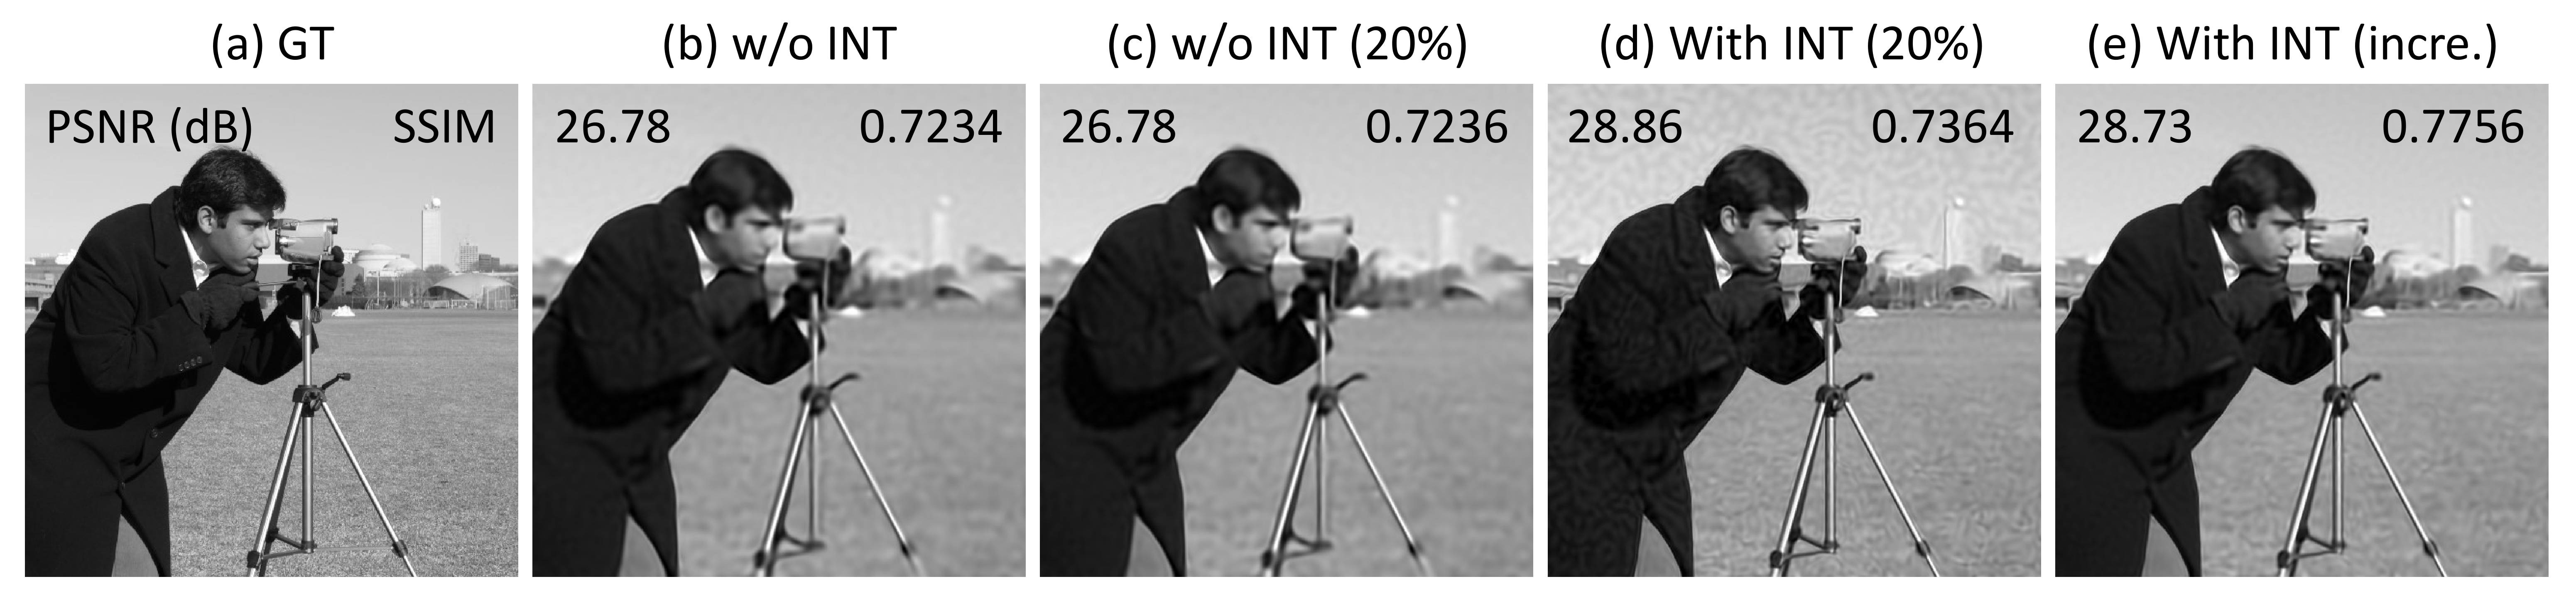
\includegraphics[width=0.5\textwidth]{out/best_pred_summary.pdf}
\caption{Reconstruction quality of SIREN. (b) trains SIREN without (w/o) INT using all pixels. (c) trains it w/o INT using 20\% randomly selected pixels. (d) trains it using INT of 20\% selection rate. (e) trains it using progressive INT (\ie, increasing selection rate progressively from 20\% to 100\%).}
\end{figure}

\begin{itemize}
    \item {\bf INT on multiple real-world modalities.}
\end{itemize}

The encoding time is measured excluding data I/O latency.

\begin{figure}
    \centering
    \includegraphics[width=0.6\textwidth]{Source/intTable.pdf}
\end{figure}

\end{block}
\end{column}

\end{columns}
\end{frame}

\end{document}

%%%%%%%%%%%%%%%%%%%%%%%%%%%%%%%%%%%%%%%%%%%%%%%%%%%%%%%%%%%%%%%%%%%%%%%%%%%%%%%%%%%%%%%%%%%%%%%%%%%%
%%% Local Variables: 
%%% mode: latex
%%% TeX-PDF-mode: t
%%% End: 